\chapter{Theoretical Background}

\section{Physics of MRI}
\subsection{Components of MRI machines}
The theory of measurements based on nuclear magnetic resonance has its root in quantum physics: The nuclear magnetic moment and the angular momentum of protons in the atomic nuclei maintained by the spin of these particles are to be indirectly measured, and these observables depend (besides many other factors) on the tissue where the proton is located. More specifically, the MRI
machines are tuned to focus on the nucleus of protons that consist of only one proton. The core components of MRI machines are the following:
\begin{enumerate}
    \item Superconductive coils immersed in liquid helium responsible for producing a almost perfectly homogeneous and static magnetic field. The role of the liquid helium is to keep the wires at superconducting temperature, so that massive amounts of electricity can be run through the coils creating super-strong fields up to \SI{21.1}{\tesla}~\cite{schepkin_vivo_2012}. Although stronger magnetic field allows better resolution, the construction costs of such machines and the effect of the strong magnetic field on human tissues limit the strength of available MRI scanners for routine clinical from \SI{0.2}{\tesla} to \SI{3.0}{\tesla}, and up to \SI{11.7}{\tesla} in research machines for human imaging~\cite{ladd_pros_2018}.
    \item Inside of this super-strong electromagnet, the so called gradient coils are located that alter the field along all three dimensions creating spatially varying magnetic field (hence the name: gradient coils) in order of \SI{}{\milli\tesla}, so that signals coming from different location within the coils are possible to be separated. They are also used to provide contrast for diffusion and flow imaging.
    \item Within the Radio Frequency (RF) coils are located that emit and measure time varying electromagnetic signals on order of tens of \SI{}{\micro\tesla}.
\end{enumerate}
The reason behind this elaborate design (depicted on fig.~\ref{fig:mri_schematic}) is the need of creating a measurement setup suitable to give a very fine control over the the direction of the magnetic moment of protons of hydrogen atoms within the measured object (which, in our case, is the human body that contains a large amount of hydrogen mostly in the form of water, but also bounded within other molecules).

\subsection{Macroscopic Magnetization}
The purpose of the superconductive coils is to align the magnetic moment of protons with the direction of the magnetic field. This direction (also corresponding to the head-to-foot direction) is usually referred as longitudinal direction or z direction, and the plane perpendicular to this direction is called the transverse plane or the x-y plane. This alignment of the magnetic moment of the protons leads to two configurations: protons with their magnetic moment pointing to the same direction as the static magnetic field, and other protons having their magnetic moment with opposite direction. Without the static field, the randomly oriented spins cancel out each other, as they also do in the aligned case, when the number of protons oriented to the two directions are equal. But in real systems, a slight excess of the protons aligned with the static magnetic field always produces a net magnetization with the same direction as the external magnetic field.

The ratio of the number of protons in these two groups are described by the Fermi-Dirac statistics. In strong and static magnetic field at room temperature, the Fermi-Dirac distribution reduces to Boltzmann distribution resulting the following formula:
\[N_+ = N \cdot \frac{e^{E_+ / (k_B T)}}{e^{E_+ / (k_B T)} + e^{E_- / (k_B T)}} \text{ and } N_- = N \cdot \frac{e^{E_- / (k_B T)}}{e^{E_+ / (k_B T)} + e^{E_- / (k_B T)}},\]
where $N$ is the total number of protons, $N_+$ and $N_-$ are the numbers of protons pointing to the same and opposite direction as the static magnetic field, $E_+$ and $E_-$ are their respective energy levels, $k_B$ is the Boltzmann-constant, and $T$ is the temperature. In this case neighboring energy levels are equidistant with the difference in the secondary spin quantum number of $\Delta m = \pm 1$ and the energy difference of $\nabla E = \gamma \hbar B_0$, where $\gamma$ is an empirical constant called gyromagnetic ratio (equals to $42.575 \cdot 2\pi$\SI{}{\mega\hertz/\tesla} in case of protons), $\hbar$ is the reduced Planck constant, and $B_0$ is the static external magnetic field. The ratio of Boltzmann distributions for two states a spin \textonehalf nucleus is known as the Boltzmann factor:
\[f(E) = e^{-\frac{\gamma \hbar B_0}{k_B T}}.\]
Using this factor, the ratio of unpaired protons (these protons give the net magnetization) divided by the number of all protons is given by
\[\frac{N_+ - N_-}{N_+ + N_-} = \frac{\gamma \hbar B_0}{2 k_B T}.\]
This ratio at room temperature in a static field with a couple teslas tends to be a tiny number (in the order of \num{1e-6} multiplied by $B_0$), so that explains why do MRI machines need such a strong electromagnets. (Note that this ratio also can be increased by increasing the temperature, but it is not feasible for human imaging.)

\begin{figure}
    \centering
    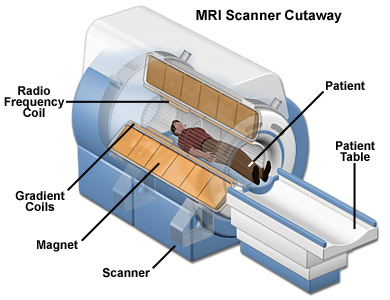
\includegraphics[width=0.45\textwidth]{images/mri-scanner.jpg}
    \caption{Schematic illustration of construction of a cylindrical MRI scanner.\\
    Source: Adapted from~\cite{coyne_mri_2020}}
    \label{fig:mri_schematic}
\end{figure}

\subsection{Precession}
In equilibrium when all protons are aligned with the external magnetic field, the longitudinal component of net magnetization is maximal and the component in the transverse plane is zero. However, with the aid of an electromagnetic excitation in the transverse plane emitted by the RF coils, it is possible to rotate the vector of net magnetization into the transverse plane. The key factor in this process is to tune the frequency of the excitation to match the so called precessional frequency of the protons given by the Larmor equation:
\[\omega = \gamma B_0.\]
The name \textit{precessional frequency} comes from the phenomenon that the magnetic moment of protons start to \textit{precess} around the longitudinal axis (which, again, is the direction of static external magnetic field) due to its intrinsic angular momentum. When the frequency of the excitation matches the precessional frequency of the proton (which happens to be in the radio frequency range, hence the name of RF coils), then resonance occurs and the angle of net magnetization gets tilted, otherwise the electromagnetic field has little to no effect of the net magnetization. An RF excitation of a duration $\tau$ causes rotation of the magnetization by an angle $\theta$, which is called the flip angle, defined by
\[\theta = \gamma \int_0^\tau B_1(t) dt = \gamma \tau B_1,\]
where $B_1$ is the magnetization of RF excitation, and it is assumed to be constant over time window of excitation with length $\tau$.

As a result of the precession, the net magnetic flux changes in the RF coils (these coils used for both emitting and receiving RF signals) inducing an electromotive force $U_{ind}$ that can be calculated by Faraday's law of induction:
\[U_{ind} = -\frac{d\Phi}{dt}.\]
Projecting the precessing movement (with the Larmor frequency $\omega$) of the net magnetization to transversal plan, we get a sinusoidal change in flux that results in the following formula:
\[U_{ind} \sim sin(\theta)\, \omega\, cos(\omega t) = sin(\theta)\, \gamma\, B_0\, cos(\gamma\, B_0\ t).\]
While this formula is not an exact model that fits the current measured in the RF coils, but it captures three important aspects of the resulted electric signal:
\begin{enumerate}
    \item It is a sinusoidal signal with a frequency depending only on a constant specific to protons and the external magnetic field.
    \item The amplitude of that signal depends on the flip angle induced by an RF excitation.
    \item And it is also dependent on the external magnetic field (yet another reason why MRI machines need very strong electromagnets).
\end{enumerate}

\subsection{Relaxation}
For a more accurate model, one should consider that as the protons emit RF signal due to their precessing magnetic moment, they lose the energy of the excitation and they slowly return to the low energy state; i.e., to the state where the magnetic moment of protons are aligned along the longitudinal axis, and where the net magnetization points to the same direction as the external field. Assuming that the excitation resulted in a perpendicular flip angle, the longitudinal component of magnetization is characterized by the exponential formula
\[M_z = M_0 (1 - e^{-t/T_1}),\]
where $M_0$ is the amplitude of magnetization in the equilibrium and is often called Boltzmann magnetization, and $T_1$ time constant is a property of the protons dependent on the tissue where they are located. This process is usually referred as $T_1$ relaxation.

Furthermore, the net magnetization is also affected by another relaxation process referred as $T_2$ relaxation. The phenomenon causing this relaxation is called \textit{dephasing}, and the name comes from the fact that when excitation is applied to protons in the equilibrium, they will precess in the same phase, but soon they lose this synchronization. This desynchronization is due to the slight inhomogeneity of the static external field caused by four factors: spin-spin interactions (quantum mechanical interactions with the nearby protons), magnetic field inhomogeneities (hardware limitations), magnetic susceptibility (slight magnetization of molecules within the measured part of the body), and chemical shift effects (shielding effect of the electron cloud of molecules incorporating the hydrogen atoms). The slightly different $B_0$ value makes the Larmor frequency different, and that results in the desynchronization of phase. The outcome of this process is that the transversal component of the net magnetization decays exponentially to zero. The speed of decay is characterized by the $T_2^*$ time constant:
\[M_{xy} = M_1\,e^{-t/T_2^*},\]
where $M_1$ is the initial amplitude of net magnetization in the beginning of the $T_2$ relaxation process. Using, however, the later described \textit{spin-echo} measurement protocol, the last three inhomogeneity-causing factors can be cancelled out leading to a slightly different time constant denoted by $T_2$.

\subsection{MRI Sequences}
Although the theory explained above are always the same for all MRI measurements, numerous methods exist and are used in today's medicine producing drastically different. These methods are usually referred as MRI sequences and they mostly differ in the a particular setting of RF pulses and the gradients in the static magnetic field, resulting in a particular image appearance. The most commonly used group of MRI sequences is the \textit{spin echo}~\cite{hahn_spin_1950}. In accordance with the two types of relaxation, sequences in that group have two main parameters: $TR$ (Time of Repetition) and $TE$ (Time of Echo). These parameters have a crucial role timing the recording of current in the RF coils when the difference between the amplitude of the RF signal emitted by the excited protons is maximal because this difference makes it possible later to distinguish different tissues.

The $TR$ parameter is connected to the $T_1$ value, as it determines the time between two excitation pulses. Having a larger $TR$ value allows protons to get better aligned with the external magnetic field before the next excitation, which results in a higher initial value for $M_{xy}$, leading to a stronger current in the detector coils, but it also makes the entire measurement longer. On the other hand, $TE$ determines the delay between the peak of the RF pulse and the peak of the echo. That echo is a temporary rephasing of spins caused by a second, \SI{180}{\degree} RF pulse emitted at $t = TE/2$. That pulse inverts spins, and therefore it makes spins with slower Larmor frequency, which lagged behind the faster ones previously, be ahead of the others in phase. At the time when faster precessing protons catch up, the transversal magnetization exhibits an echo peak. As stated earlier, an important advantage of spin echo technique is that three factors of magnetic inhomogeneity is cancelled out by the inversion as these factors are constant over time, while spin-spin interactions are random interactions between protons that cause random local changes in the magnetic fields experienced by the protons.

Based on the choice of $TR$ and $TE$ values, we can talk about three types of spin echo sequences: $T_1$ weighted sequence has intermediate $TR$ value in the magnitude of $T_1$ producing maximal T1 weighting (at this point, the difference caused by different $T_1$ value between the amplitude of signals coming from different tissues are maximal) and short $TE$ value magnitudes smaller than $T_2$ producing minimal T2 weighting (there is not enough time to have significant difference between decay curves with different $T_2$). To the contrary, T2-weighted images have a long $TE$ (maximizing the difference in $T_2$ relaxation) and long $TR$ (reducing the weight of $T_1$ relaxation). And the third type, called proton density (PD) weighting, uses short $TE$ and long $TE$, so that the pixel intensities on the resulted image will reflect only the density of protons (that also differs between tissues), and the $T_1$ and $T_2$ values have little effect on it.

\clearpage